%%%%%%%%%%%%%%%%%%%%%%%%%%%%%%%%%%%%%%%%%%%%%%%%%%%
% val.tex
%%%%%%%%%%%%%%%%%%%%%%%%%%%%%%%%%%%%%%%%%%%%%%%%%%%
Validation of EM physics is performed on several levels.  Because EM physics is
used in practically all tests and examples, the \Gfour{} integrated test system 
routinely checks all EM physics models.  A specific EM validation suite
\cite{embib:emVal} runs on a regular basis for each reference version of \Gfour{}
(see \cite{embib:chep14,embib:chep11,embib:chep12} and references therein).
Dedicated validations of cross sections, stopping powers, and atomic transition
energies versus evaluated data and theory are done by \Gfour{} developers and 
different user groups (see, for example, 
\cite{embib:uni2,embib:valGam,embib:valGam2} and 
Figure \ref{em:compton}).  EM physics validation is also performed in various
application domains by different user communities, especially by the HEP 
experiments ATLAS and CMS. 

As an example of EM physics validation for HEP applications, the energy 
resolution of two sampling calorimeters \cite{embib:uni3,embib:uni4} 
versus the cut in range value and \Gfour{} version is shown in 
Figure~\ref{Figure-UEM1}.  This plot illustrates the good agreement of \Gfour{}
simulation predictions with data, and the stability between \Gfour{} versions of 
simulation results for high energy physics applications.

\begin{figure}
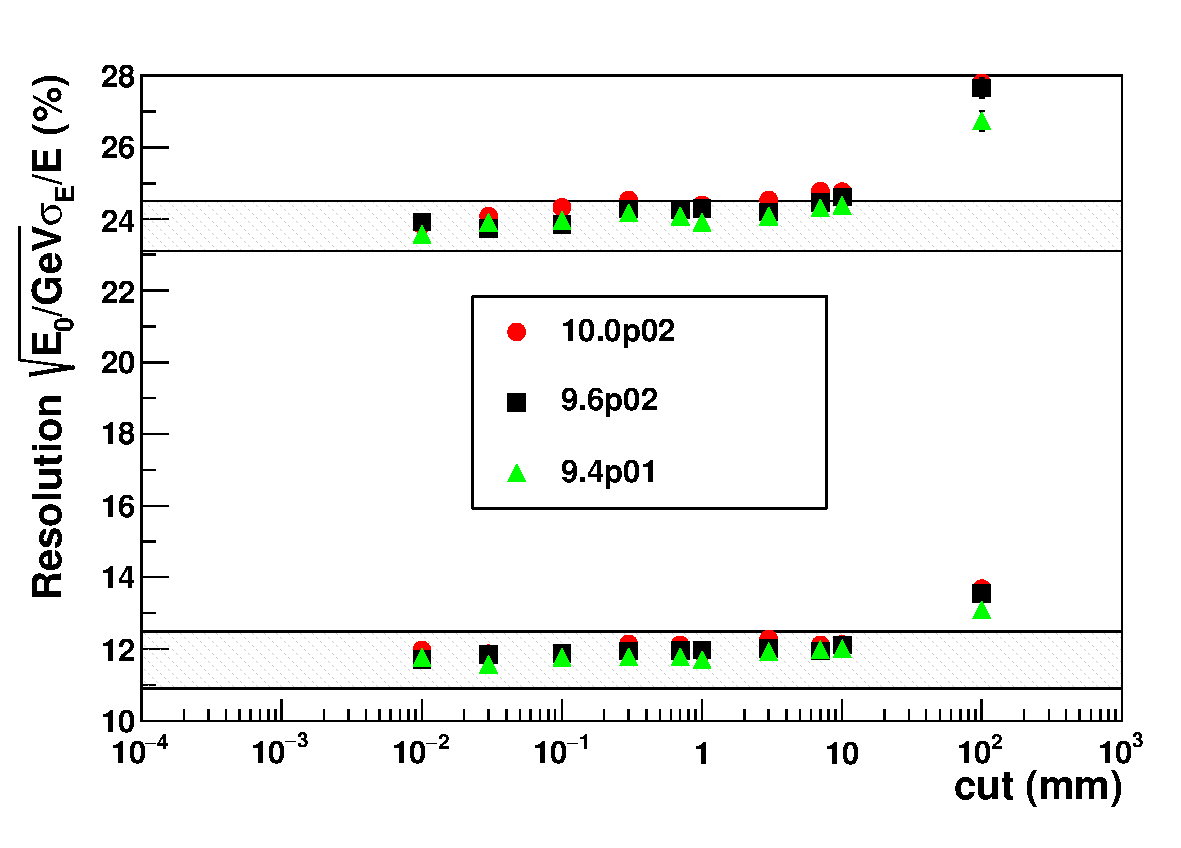
\includegraphics[width=0.5\textwidth]{figures/Azeus.pdf}
\caption{Energy resolution of two sampling Lead/Scintillator calorimeters 
for 10 GeV electrons: squares, circles and triangles indicate \Gfour{} 
simulations for different versions of the toolkit, and each band indicates 
experimental data with one standard deviation uncertainty
\cite{embib:uni3,embib:uni4}.}
\label{Figure-UEM1}
\end{figure}

Further validations come from the medical and space communities, in particular, 
GATE \cite{embib:GATE}, GAMOS \cite{embib:GAMOS}, GRAS \cite{embib:gras}, 
and TOPAS \cite{embib:TOPAS}.
There are also many validation results obtained by single user groups.  For 
example, validations for space shielding were done recently in 
\cite{embib:elshield} and for therapeutic ion beam simulation in 
\cite{embib:emIonUser}.

%end
